\section{Written Questions [35pts]}
\label{sec:written}

Answer the following questions in the HW2 solutions template provided. DO NOT show your work. Then upload your solutions to Gradescope.

\subsection{Gini Impurity}
\label{sec:gini}

First, let's think a little bit about decision trees. The following dataset $D$ consists of 7 examples, each with 3 attributes, $(A,B,C)$, and a label, $Y$.

\begin{center}
\begin{tabular}{|c|c|c|c|}
\hline
$A$ & $B$ & $C$ & $Y$ \\ \hline
1 & 1 & 0 & 0     \\ \hline
1 & 1 & 2 & 1     \\ \hline
1 & 0 & 0 & 1     \\ \hline
1 & 1 & 2 & 1     \\ \hline
0 & 0 & 2 & 0     \\ \hline
0 & 1 & 1 & 0     \\ \hline
0 & 0 & 0 & 0     \\ \hline
\end{tabular}
\end{center}


Use the data above to answer the following questions. 

\begin{notebox}
A few important notes:
\begin{itemize}
    \item \emph{All calculations should be done without rounding!} After you have finished all of your calculations, write your rounded solutions in the boxes below.
    %\item Unless otherwise noted, numeric solutions should include 4 digits of precision (e.g. 0.1234).
    \item Note that, throughout this homework, we will use the convention that the leaves of the trees do not count as nodes, and as such are not included in calculations of depth and number of splits. (For example, a tree which classifies the data based on the value of a single attribute will have depth 1, and contain 1 split.)
\end{itemize}
\end{notebox}

\begin{questions}
    \question[1] What is the Gini impurity of $Y$, $G(Y;D)$, before any splitting happens?
    %
    (Please include one number rounded to the fourth decimal place, e.g. 0.1234)
    
    \begin{tcolorbox}[fit,height=1cm, width=2cm, blank, borderline={1pt}{-2pt},nobeforeafter]
    %solution 
    \end{tcolorbox}
    
    
    
    \question[1] What is the resulting Gini gain on $Y$ if we were to split on $A$, i.e. $G(Y,A;D)$?
    %
    (Please include one number rounded to the fourth decimal place, e.g. 0.1234)
    
    \begin{tcolorbox}[fit,height=1cm, width=2cm, blank, borderline={1pt}{-2pt},nobeforeafter]
    %solution 
    \end{tcolorbox}
    
    

    \question[1] What is the resulting Gini gain on $Y$ if we were to split on $B$, i.e. $G(Y,B;D)$?
    %
    (Please include one number rounded to the fourth decimal place, e.g. 0.1234)
    
    \begin{tcolorbox}[fit,height=1cm, width=2cm, blank, borderline={1pt}{-2pt},nobeforeafter]
    %solution 
    \end{tcolorbox}
    
    
    
    \question[1] What is the resulting Gini gain on $Y$ if we were to split on $C$, i.e. $G(Y,C;D)$?
    %
    (Please include one number rounded to the fourth decimal place, e.g. 0.1234)
    
    \begin{tcolorbox}[fit,height=1cm, width=2cm, blank, borderline={1pt}{-2pt},nobeforeafter]
    %solution 
    \end{tcolorbox}
    
    
    
   \question[1] Consider the dataset given above. Which attribute ($A$, $B$, or $C$) would a decision tree algorithm pick first to branch on, if its splitting criterion is Gini impurity?
    
    \textbf{Select one:}
    \begin{checkboxes}
        \choice $A$
        \choice $B$
        \choice $C$
    \end{checkboxes}
    
    
    
    \question[1] Consider the dataset given above. Which is the second attribute you would pick to branch on, if its splitting criterion is Gini impurity? (\emph{Hint:} Notice that this question correctly presupposes that there is \emph{exactly one} second attribute.)
    
    \textbf{Select one:}
    \begin{checkboxes}
        \choice $A$
        \choice $B$
        \choice $C$
    \end{checkboxes}
    
    
    \question[1] If the same algorithm continues until the tree perfectly classifies the data, what would the depth of the tree be?
    
    \begin{tcolorbox}[fit,height=1cm, width=2cm, blank, borderline={1pt}{-2pt},nobeforeafter]
    %solution 
    \end{tcolorbox}
    
    
\clearpage
    \question[4] Draw your completed Decision Tree. Label the non-leaf nodes with which attribute the tree will split on (e.g. $B$), the edges with the value of the attribute (e.g. 1 or 0), and the leaf nodes with the classification decision (e.g. $Y=0$).
    
    \begin{tcolorbox}[fit,height=20cm, width=15cm, blank, borderline={1pt}{-2pt},nobeforeafter]
    %solution 
    \end{tcolorbox}
    

\end{questions}

\subsection{Mutual Information}
\label{sec:mutual information}

Now, using the same dataset, let's consider another splitting criterion, Mutual Information.

\begin{center}
\begin{tabular}{|c|c|c|c|}
\hline
$A$ & $B$ & $C$ & $Y$ \\ \hline
1 & 1 & 0 & 0     \\ \hline
1 & 1 & 2 & 1     \\ \hline
1 & 0 & 0 & 1     \\ \hline
1 & 1 & 2 & 1     \\ \hline
0 & 0 & 2 & 0     \\ \hline
0 & 1 & 1 & 0     \\ \hline
0 & 0 & 0 & 0     \\ \hline
\end{tabular}
\end{center}


Use the data above to answer the following questions. 

\begin{questions}
    \question[1] What is the entropy of $Y$ in bits, $H(Y)$? In this and subsequent questions, when we request the units in \emph{bits}, this simply means that you need to use $\log$ base 2 in your calculations.\footnote{If instead you used $\log$ base $e$, the units would be \emph{nats}; $\log$ base 10 gives \emph{bats}.}
    %
    (Please include one number rounded to the fourth decimal place, e.g. 0.1234)
    
    \begin{tcolorbox}[fit,height=1cm, width=2cm, blank, borderline={1pt}{-2pt},nobeforeafter]
    %solution 
    \end{tcolorbox}
    
    
    \question[1] What is the mutual information\footnote{In the context of decision trees, and therefore in this assignment, the terms ``information gain" and ``mutual information" are synonymous (e.g. they have the same meaning as one another). However, in information theory and machine learning in general, ``information gain" is synonymous with ``Kullback-Leibler (K-L) divergence", often referred to as relative entropy, which is not the same as mutual information. For more information, go \href{https://en.wikipedia.org/wiki/Information_gain_in_decision_trees}{here.} } 
    of $Y$ and $A$ in bits, $I(Y; A)$?
    %
    (Please include one number rounded to the fourth decimal place, e.g. 0.1234)
    
    \begin{tcolorbox}[fit,height=1cm, width=2cm, blank, borderline={1pt}{-2pt},nobeforeafter]
    %solution 
    \end{tcolorbox}
    

    \question[1] What is the mutual information of $Y$ and $B$ in bits, $I(Y; B)$?
    %
    (Please include one number rounded to the fourth decimal place, e.g. 0.1234)
    
    \begin{tcolorbox}[fit,height=1cm, width=2cm, blank, borderline={1pt}{-2pt},nobeforeafter]
    %solution 
    \end{tcolorbox}
    
    
    \question[1] What is the mutual information of $Y$ and $C$ in bits, $I(Y; C)$?
    %
    (Please include one number rounded to the fourth decimal place, e.g. 0.1234)
    
    \begin{tcolorbox}[fit,height=1cm, width=2cm, blank, borderline={1pt}{-2pt},nobeforeafter]
    %solution 
    \end{tcolorbox}
    

\clearpage

    \question[1] Consider the dataset given above. Which attribute ($A$, $B$, or $C$) would a decision tree algorithm pick first to branch on, if its splitting criterion is mutual information?
    
    \textbf{Select one:}
    \begin{checkboxes}
        \choice $A$
        \choice $B$
        \choice $C$
    \end{checkboxes}
    
    
    \question[3] Is the resulting tree the same as if we split using Gini Impurity? Explain in your own words what Gini Impurity and Mutual Information are each calculating.
    
    \begin{tcolorbox}[fit,height=7cm, width=15cm, blank, borderline={1pt}{-2pt},nobeforeafter]
    %solution 
    \end{tcolorbox}
    

\end{questions}

\clearpage
\subsection{Empirical Questions}
\label{sec:empirical}

The following questions should be completed as you work through the programming portion of this assignment (Section \ref{sec:programming}).

 \begin{questions}
    \question[2] Train and test your decision tree on the politician dataset and the education dataset with four different values of max-depth, $\{0,1,2,4\}$. Report your findings in the HW2 solutions template provided. A Decision Tree with max-depth 0 is simply a \emph{majority vote classifier}; a Decision Tree with max-depth 1 is called a \emph{decision stump}. If desired, you could even check that your answers for these two simple cases are correct using your favorite spreadsheet application (e.g. Excel, Google Sheets). (Please round each number to the fourth decimal place, e.g. 0.1234)
    
    \begin{center}
    \begin{tabular}{cc|c|c}
        \toprule
      {\bf Dataset}   & {\bf Max-Depth} & {\bf Train Error} & {\bf Test Error} \\
      \midrule
        politician & 0 & & \\
        politician & 1 & & \\
        politician & 2 & & \\
        politician & 4 & & \\
        \midrule
        education & 0 & & \\
        education & 1 & & \\
        education & 2 & & \\
        education & 4 & & \\
        \bottomrule
    \end{tabular}
    \end{center}
    
    
    \question[3] For the politicians dataset, create a computer-generated plot showing error on the y-axis against depth of the tree on the x-axis. Plot \emph{both} training error and testing error, clearly labeling which is which.  That is, for each possible value of max-depth ($0, 1, 2, \ldots,$ up to the number of attributes in the dataset), you should train a decision tree and report train/test error of the model's predictions.
    
    \begin{tcolorbox}[fit,height=10cm, width=15cm, blank, borderline={1pt}{-2pt},nobeforeafter]
    %solution 
    \end{tcolorbox}
    

\clearpage
    \question[2] Suppose your research advisor asks you to run some model selection experiments and then report your results. You select the Decision Tree model's max-depth to be the one with lowest test error in metrics.txt and then report that model's test error as the performance of our classifier on held out test data. Is this a good experimental setup? If so, why? If not, why not?
    
    \begin{tcolorbox}[fit,height=8cm, width=15cm, blank, borderline={1pt}{-2pt},nobeforeafter]
    %solution 
    \end{tcolorbox}
    


    \question[2] In this assignment, we used max-depth as our stopping criterion, and as a mechanism to prevent overfitting. Alternatively, we could stop splitting a node whenever the gini gain for the best attribute is lower than a threshold value. This threshold would be another hyperparameter. Theoretically, how would increasing this threshold value affect the number of nodes and depth of the learned trees?
    
    \begin{tcolorbox}[fit,height=8cm, width=15cm, blank, borderline={1pt}{-2pt},nobeforeafter]
    %solution 
    \end{tcolorbox}
    


\clearpage
    \question[2] From section 1.3 question 4, how would you set-up model training to choose the threshold value?
    
    \begin{tcolorbox}[fit,height=10cm, width=15cm, blank, borderline={1pt}{-2pt},nobeforeafter]
    %solution 
    \end{tcolorbox}
    

    
\clearpage
    \question[3] Print (do not handwrite!) the decision tree which is produced by your algorithm for the politician data with max depth 3. Instructions on how to print the tree could be found in section \ref{sec:printtree}.
    
    \begin{tcolorbox}[fit,height=19cm, width=15cm, blank, borderline={1pt}{-2pt},nobeforeafter]
    %solution 
    

    
    \end{tcolorbox}
    
    
    
    \clearpage
    \question[2] Below is the printed decision tree for the previous problem when the splitting criteria is Mutual Information instead of Gini impurity. Compare the two and comment on the differences.
    \begin{figure}[H]
    \begin{center}
    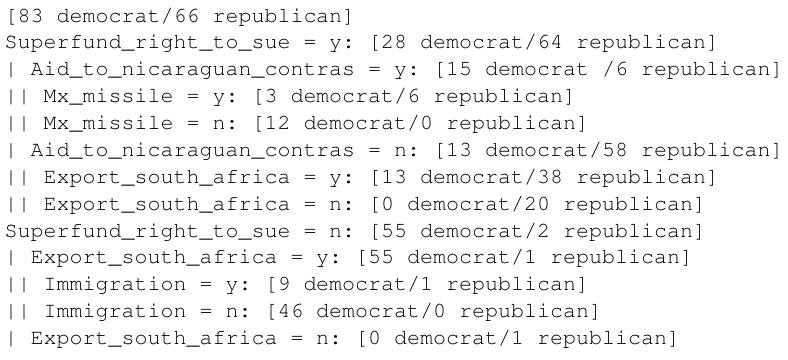
\includegraphics[scale=1]{images/mutual.png}
    \end{center}
    \end{figure}
    
    \begin{tcolorbox}[fit,height=13cm, width=15cm, blank, borderline={1pt}{-2pt},nobeforeafter]
    %solution 
    \end{tcolorbox}
    

    
    
    \clearpage
    \question After you have completed all other components of this assignment, report your answers to the collaboration policy questions detailed in the Academic Integrity Policies found \href{http://www.cs.cmu.edu/~mgormley/courses/10601bd-f18/about.html#7-academic-integrity-policies}{here}.
    \begin{enumerate*}
        \item Did you receive any help whatsoever from anyone in solving this assignment? Is so, include full details.
        \item Did you give any help whatsoever to anyone in solving this assignment? Is so, include full details.
        \item Did you find or come across code that implements any part of this assignment ? If so, include full details.
    \end{enumerate*}
    
    \begin{tcolorbox}[fit,height=19cm, width=15cm, blank, borderline={1pt}{-2pt},nobeforeafter]
    %solution 
    \end{tcolorbox}
    
\end{questions}

